\documentclass{article}
\pagestyle{empty}
\usepackage{tikz}
\usepackage{caption}
\usepackage{subcaption}
\usepackage{graphicx}

\begin{document}
\usetikzlibrary{positioning,shapes}
\definecolor{yellowish}{HTML}{FFE699}
\definecolor{grayish}{HTML}{D9D9D9} 
\tikzset{
   rect/.style={
      align=center,
      text=black,    
      minimum width=2.5cm,
      minimum height=2cm}
}
\tikzset{
   done/.style={rect, fill=grayish }
}
\tikzset{
   todo/.style={rect, fill=yellowish}
}
\tikzset{
   arrow/.style={line width=1mm}
}
\definecolor{babyblueeyes}{rgb}{0.36, 0.61, 0.83}

\centering
\begin{figure}[ht]
   \centering
   \begin{subfigure}[b]{0.4\textwidth}
      \centering
      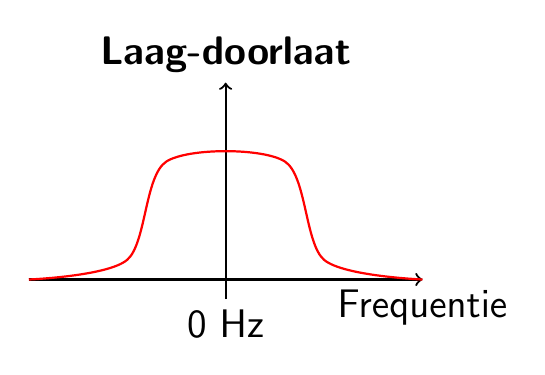
\begin{tikzpicture}[scale=0.5, font=\sffamily\Large] 
         \draw[->, thick] (-5,0) -- (5,0) node[below]{Frequentie};
         \draw[->, thick] (0,-0.5) node[below]{0 Hz} -- (0,5) node[above]{\textbf{Laag-doorlaat}};
         \draw[red, thick, smooth] plot[tension=0.5] coordinates{(-5,0) (-2.5,0.5) (-1.5,3) (1.5,3) (2.5,0.5) (5,0)};
      \end{tikzpicture}
   \end{subfigure}
   \hfill
   \begin{subfigure}[b]{0.4\textwidth}
      \centering
      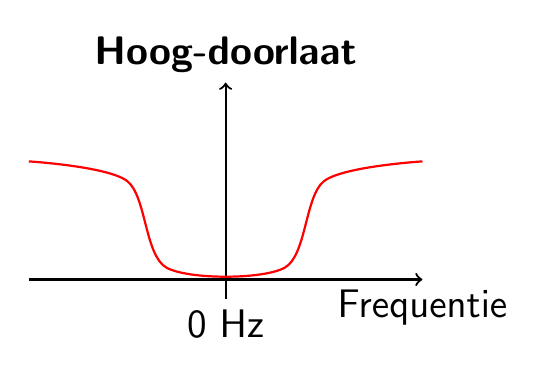
\begin{tikzpicture}[scale=0.5, font=\sffamily\Large]
         \draw[->, thick] (-5,0) -- (5,0) node[below]{Frequentie};
         \draw[->, thick] (0,-0.5) node[below]{0 Hz} -- (0,5) node[above]{\textbf{Hoog-doorlaat}};
         \draw[red, thick, smooth] plot[tension=0.5] coordinates{(-5,3) (-2.5,2.5) (-1.5,0.3) (1.5,0.3) (2.5,2.5) (5,3)};
      \end{tikzpicture}
   \end{subfigure}   

   \begin{subfigure}[b]{0.4\textwidth}
      \centering
      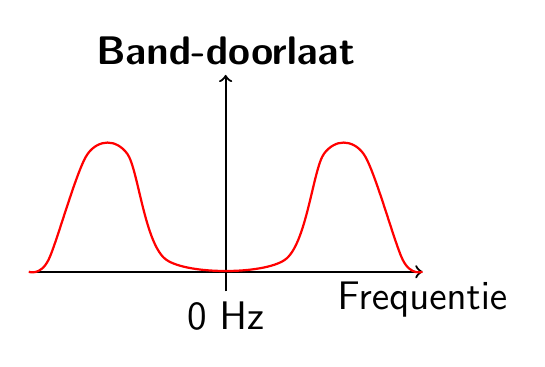
\begin{tikzpicture}[scale=0.5, font=\sffamily\Large] 
         \draw[->, thick] (-5,0) -- (5,0) node[below]{Frequentie};
         \draw[->, thick] (0,-0.5) node[below]{0 Hz} -- (0,5) node[above]{\textbf{Band-doorlaat}};
         \draw[red, thick, smooth] plot[tension=0.5] coordinates{(-5,0) (-4.5,0.3) (-3.5,3) (-2.5,3) (-1.5,0.3) (1.5, 0.3) (2.5,3) (3.5, 3) (4.5,0.3) (5,0)};
      \end{tikzpicture}
   \end{subfigure}
   \hfill
   \begin{subfigure}[b]{0.4\textwidth}
      \centering
      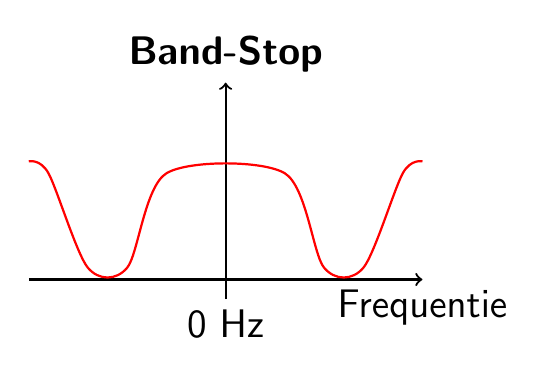
\begin{tikzpicture}[scale=0.5, font=\sffamily\Large]
         \draw[->, thick] (-5,0) -- (5,0) node[below]{Frequentie};
         \draw[->, thick] (0,-0.5) node[below]{0 Hz} -- (0,5) node[above]{\textbf{Band-Stop}};
         \draw[red, thick, smooth] plot[tension=0.5] coordinates{(-5,3) (-4.5,2.7) (-3.5,0.3) (-2.5,0.3) (-1.5,2.7) (1.5, 2.7) (2.5,0.3) (3.5, 0.3) (4.5,2.7) (5,3)};   
      \end{tikzpicture}
   \end{subfigure}
\end{figure}

\end{document}